\documentclass[letterpaper,twocolumn,10pt]{article}
\usepackage{vendor/usenix2019_v3}
\usepackage{graphicx,booktabs,amsmath}
\usepackage{dblfloatfix}
\renewcommand{\topfraction}{0.90}
\renewcommand{\dbltopfraction}{0.90}
\renewcommand{\textfraction}{0.08}
\renewcommand{\floatpagefraction}{0.75}
\renewcommand{\dblfloatpagefraction}{0.75}
\setcounter{topnumber}{3}
\setcounter{dbltopnumber}{3}
\graphicspath{{figures/}}
\pagestyle{plain}
\hypersetup{colorlinks=true,allcolors=black,pdftitle={GPUOS: An Operating-System Architecture for Shared GPU Execution}}
\newcommand{\system}{GPUOS}
\newcommand{\res}[1]{\csname result#1\endcsname}
\expandafter\def\csname resultNative32\endcsname{143.3}
\expandafter\def\csname resultPersistent32\endcsname{117.9}
\expandafter\def\csname resultCLC32\endcsname{113.2}
\expandafter\def\csname resultFixed32\endcsname{121.3}
\expandafter\def\csname resultRequestGain32\endcsname{1.215}
\expandafter\def\csname resultRequestReduction32\endcsname{17.7}
\expandafter\def\csname resultNative64\endcsname{274.9}
\expandafter\def\csname resultPersistent64\endcsname{225.0}
\expandafter\def\csname resultCLC64\endcsname{215.2}
\expandafter\def\csname resultFixed64\endcsname{232.0}
\expandafter\def\csname resultRequestGain64\endcsname{1.222}
\expandafter\def\csname resultRequestReduction64\endcsname{18.2}
\expandafter\def\csname resultMaxRequestNRMSE\endcsname{0.007762}
\expandafter\def\csname resultMaxReplayNRMSE\endcsname{0.008308}
\expandafter\def\csname resultplacementGeo\endcsname{1.234}
\expandafter\def\csname resultplacementMax\endcsname{1.925}
\expandafter\def\csname resultpartitionGeo\endcsname{1.843}
\expandafter\def\csname resultpartitionMax\endcsname{3.988}
\expandafter\def\csname resultfusionGeo\endcsname{0.994}
\expandafter\def\csname resultfusionMax\endcsname{1.074}
\expandafter\def\csname resultTmaFourGeo\endcsname{1.008}
\expandafter\def\csname resultnew_request_samples\endcsname{150.0}
\expandafter\def\csname resultnew_replay_samples\endcsname{315.0}

\newcommand{\slackProxyShortCost}{0.62}
\newcommand{\slackProxyShortRate}{0.741}
\newcommand{\slackProxyShortFraction}{6.507}
\newcommand{\slackProxyMediumCost}{2.50}
\newcommand{\slackProxyMediumRate}{1.167}
\newcommand{\slackProxyMediumFraction}{10.213}
\newcommand{\slackProxyLongCost}{23.68}
\newcommand{\slackProxyLongRate}{4.359}
\newcommand{\slackProxyLongFraction}{38.252}
\newcommand{\slackContinuousCost}{3.48}
\newcommand{\slackContinuousRate}{0.374}
\newcommand{\slackContinuousFraction}{3.276}
\newcommand{\slackModelMediumCost}{-3.04}
\newcommand{\slackModelMediumRate}{0.039}
\newcommand{\slackModelMediumFraction}{0.342}
\newcommand{\slackModelLongCost}{-1.57}
\newcommand{\slackModelLongRate}{8.779}
\newcommand{\slackModelLongFraction}{76.999}
\newcommand{\slackTimedSteps}{154,368}
\newcommand{\slackAdmissionPasses}{9}
\newcommand{\slackAdmissionCount}{9}
\newcommand{\slackPauseShort}{10.69}
\newcommand{\slackPauseMedium}{21.85}
\newcommand{\slackPauseLong}{738.68}

\date{}
\title{\Large\bf GPUOS: An Operating-System Architecture\\for Shared GPU Execution}
\author{\rm Working draft}
\begin{document}
\maketitle
\begin{abstract}
Latency-sensitive inference can leave arithmetic capacity idle while occupying
resources needed by other GPU work. Recovering that capacity requires a
contract for interference, suspension, and resource return. Building on
\emph{The GPU Needs an Operating System}, we specify GPUOS, an architecture
that represents execution as restartable tasks admitted under revocable
resource leases. Its six layers connect compiler safe points, device dispatch,
resource governance, interference estimates, and slack-aware admission.
The design separates cooperative suspension, finite kernel slices, and
driver-managed context switching, and identifies hardware services needed
for enforceable pause and memory-quality guarantees.
Component prototypes provide evidence on one 32-GB RTX 5090: bounded fused
inference, a restricted FX-to-Triton compiler, cooperative background work,
and cross-process admission. Qualified fused search reduces complete-request
latency by \res{RequestReduction32}\% and \res{RequestReduction64}\%
against native cached execution, while a matched CLC+PDL control remains
faster. A streaming proxy admits \slackProxyMediumRate{} TFLOP/s of background
work at \slackProxyMediumCost\% foreground p99 cost, but whole-step suspension
recovers little work beside full-model replay. These measurements support
selected mechanisms rather than a completed general-purpose implementation.
The paper presents a unified system specification, its implemented subset,
and the remaining compiler, service, and hardware requirements.
\end{abstract}

\section{Introduction}
\label{sec:intro}
The useful unit of GPU ownership is rarely an entire device for the entire
lifetime of an application. A model server needs a prompt response at some
moments, a large KV allocation at others, and sustained memory throughput
during decode. An adapter update or an evaluation job may tolerate interruption
while consuming the arithmetic capacity that the server leaves available.
Assigning the same indivisible device to either application hides these
differences. Sharing the device without controlling interference can be worse:
a throughput improvement is not useful if an interactive request misses its
response-time objective.

Nourai and Bastani's \emph{The GPU Needs an Operating System} makes this case
through large-model measurements and a hardware--software research agenda
\cite{Nourai2026GPUOS}. We adopt its central organizing idea: GPU resources
should be granted according to the urgent workload's remaining slack, rather
than treating low average utilization as unconditional permission to run more
work. We develop that idea into an architectural specification for \system{},
covering process state, resource contracts, compiler checkpoints, admission,
revocation, memory leases, and the hardware interface. This is a system-design
paper supported by component experiments. The architecture includes services
that the current prototype does not yet implement; the implementation and
evaluation identify that boundary explicitly.

The resulting abstraction is a \emph{resource lease attached to restartable
work}. A lease specifies which resources a task may consume, how its progress
is committed, and how much revocation delay admission must reserve. A task can
run in a fused device executor, as a sequence of compiler-generated kernel
slices, or in a separate protected CUDA context. These are execution backends
with different costs and guarantees, not interchangeable meanings of
preemption. The architecture chooses among them using a workload-specific
cost model and preserves one accounting interface across the alternatives.

The prototype results expose limits as well as opportunities. Qualified
fused search improves on native cached execution, but matched CLC+PDL
remains faster. Cooperative sharing benefits a streaming proxy, while
whole-step suspension yields little work beside full-model replay.
The OS must therefore be able to reject an elaborate scheduling path
when ordinary co-running is better.

Our contribution is an explicit architectural specification, an execution
contract separating checkpoint safety from resource return, and component
evidence for bounded implementations. The resource-vector and slack-driven
sharing ideas originate in the cited work; new hardware services and a
completed general-purpose implementation are not claimed.

\section{Why GPU Sharing Needs an OS Contract}
\label{sec:motivation}
\subsection{Decode and the roofline}
Consider a matrix with $W$ weights, represented by $s$ bytes per weight, and
a decode batch of $B$ tokens. A weight-only approximation performs $2BW$
floating-point operations while reading $sW$ bytes. Its arithmetic intensity
is therefore
\begin{equation}
 I_{\mathrm{weights}} = \frac{2B}{s}\quad\text{FLOP/byte}.
\end{equation}
For two-byte weights this is $B$; for one-byte weights it is $2B$. KV reads,
activation traffic, routing, and synchronization add costs that the expression
does not capture. The device ridge $R=F_{\mathrm{peak}}/\beta_{\mathrm{mem}}$
compares peak arithmetic throughput and memory bandwidth at a consistent
precision. A memory-bound operation has an idealized arithmetic-utilization
bound $\min(1,I/R)$. A low value is a structural property of the operation,
not evidence that a dispatch queue was implemented poorly.

For a mixture-of-experts layer, the relevant batch is the batch reaching one
expert. Under balanced routing, $E$ experts and $k$ active experts per token
give an average $B_e=Bk/E$. A large global batch can consequently remain a
small local matrix problem. Routing imbalance makes the average a poor
description of the tail. This matters for an OS: scheduling against the
global token count can overestimate the arithmetic reuse of each ready task,
while the latest-finishing expert determines when dependent work is released.

\paragraph{Evidence motivating the design.}
OpenInfer reports roughly 7\% tensor activity for Qwen3.5-397B at a
97.2\% deadline-attainment operating point on four RTX PRO 6000 cards,
and 2.9\% in its decode-only pool~\cite{Nourai2026GPUOS}. Its Kimi K2
experiments report 6--11\% activity at carried loads. These are that paper's
serving measurements, not our RTX 5090 observations. Its streaming control
reaches approximately 99\% of measured bandwidth on 24 of 188 SMs, whereas
its foreground reaches only about half of peak bandwidth. This contrast
motivates jointly choosing a foreground kernel and its allocation.

\subsection{Why a scheduler alone is insufficient}
Batching can increase reuse, but waiting for a larger batch consumes response
time and larger steps can increase token latency. A scheduler cannot remove
that tradeoff by rearranging identical non-preemptible kernels. It needs
additional work that is both useful and compatible with the urgent phase.
Compatibility depends on more than arithmetic intensity: a cache-resident
matrix loop and an operand-streaming GEMM may issue similar tensor work while
causing very different foreground interference.

Nor can the scheduler infer available SMs from low bandwidth utilization.
A poorly sized foreground kernel may need many SMs to generate enough
outstanding memory requests. Taking those SMs away reduces the foreground's
own throughput before the background transfers a single byte. Conversely,
a well-pipelined streaming kernel may saturate bandwidth with fewer workers.
The resource cost of a partition therefore has two parts: the foreground's
loss from a smaller execution allocation and additional interference from
the admitted background workload. The architecture measures these parts
separately whenever a suitable matched control exists.

\subsection{Time, space, and authority}
CUDA stream priorities influence scheduling but do not promise to interrupt
already-running work~\cite{CUDAStreams}. Green contexts constrain spatial
execution resources; MPS coordinates multiple clients; MIG provides a
different isolation boundary on supported devices~\cite{CUDAGreen,NVIDIAMPS}.
None should be described as a software-selected, instruction-level deadline
primitive merely because it changes latency in one workload. Hardware
context switching, compiler checkpoints, and static partitions address
different parts of the problem.

We distinguish three authorities. An application can state urgency and
declare its work. A runtime can admit or withhold future slices and manage
buffers it owns. A driver or device can enforce context and physical-resource
boundaries. The proposed OS API exposes the strongest available guarantee
without silently upgrading it. In particular, a software issue-rate limit is
not a memory-controller reservation, and a CTA launch limit is not a promise
that a particular set of SMs belongs exclusively to that client.

\section{System Architecture and Objects}
\label{sec:architecture}
\subsection{A six-layer decomposition}
We retain the source paper's six-layer decomposition as a design vocabulary
\cite{Nourai2026GPUOS}. L0 provides device signals, context scheduling,
queues, and enforceable resource controls. L1 defines the obligations of a
shareable kernel. L2 dispatches eligible work to execution resources. L3
governs resource consumption and memory capacity. L4 estimates interference
and revocation costs. L5 selects admissions within foreground slack.
Table~\ref{tab:layers} maps this specification to the current artifact.

\begin{table*}[t]
\centering\small
\begin{tabular}{p{.10\textwidth}p{.38\textwidth}p{.43\textwidth}}
\toprule
Layer & Architectural responsibility & Artifact boundary \\
\midrule
L0 & Context switch, bounded pause, resource enforcement & Existing driver switching is measured; no new device pause or memory-QoS interface. \\
L1 & Restartable work and declared resource footprint & Handwritten WMMA checkpoints and strict FX/Triton slices for supported tensor graphs. \\
L2 & Ready-work selection and dispatch & Fused per-frontier device work pool, stream-ordered worker control, and a separate host slice executor. \\
L3 & Capacity leases, issue pacing, cache/copy governance & Bounded arenas and CTA issue pacing; no physical cache or DRAM reservation. \\
L4 & Workload-specific interference and revoke-cost estimates & Measured configuration lookup; no predictor for unobserved workloads. \\
L5 & Deadline-aware admission and revocation & Held-out slack selection and one-foreground IPC admission; no integrated production service controller. \\
\bottomrule
\end{tabular}
\caption{Architectural specification and implemented evidence. The table is
a capability map, not a claim that all six layers form a finished deployed OS.}
\label{tab:layers}
\end{table*}

\subsection{Processes, tasks, and leases}
A \emph{GPU process} is the unit of ownership and accounting. Its identity
names an address-space authority, loaded executable versions, memory
allocations, and outstanding tasks. Trusted tasks may share one CUDA context
and even one fused executor; mutually untrusted tasks require a protection
boundary supplied below the runtime. The API makes this trust mode explicit
rather than treating a common function-pointer table as process isolation.

A \emph{task} names executable work and its dependency edges. Its descriptor
contains a code version, tensor views, input/output access modes, a progress
format, a resource declaration, and a deadline class. A \emph{slice} is a
bounded portion of that task with one well-defined commit boundary. A
\emph{lease} grants resources to one or more eligible slices for a bounded
interval. A lease also specifies what must happen on revocation: retain a
resident allocation, drain and return CTA resources, save to device memory,
or invoke a driver-managed context transition.

\subsection{Resource vectors and accounting}
The proposed lease resource vector is
\begin{equation}
 \mathbf r=(r_{\mathrm{SM}},r_{\mathrm{TC}},r_{\mathrm{L2}},r_{\mathrm{DRAM}},
 r_{\mathrm{cap}},r_{\mathrm{link}},r_{\mathrm{copy}},r_{\mathrm{power}}).
\end{equation}
The coordinates have different units. SM allocation concerns resident
blocks, warp issue, registers, and shared memory. Tensor work concerns
arithmetic issue. Cache and DRAM budgets concern traffic and queueing.
Capacity is bytes held over time plus the cost of reclaiming them. Link and
copy resources include direction and endpoint. Power affects clock rates
shared by otherwise disjoint work. A scalar utilization percentage cannot
substitute for this vector.

Declarations and measurements serve different purposes. A compiler can
report the logical inputs and scratch required by a slice, along with the
compiled register and shared-memory allocation. It cannot derive physical
DRAM traffic exactly from those fields because cache hits, reuse, and other
clients alter that traffic. The accounting service keeps both values, with
explicit labels. If a counter is unavailable, it remains unknown; it is not
filled with an arithmetic estimate and presented as a measurement.

Resource prices are foreground costs, not universal exchange rates. For
foreground class $f$, background declaration $\mathbf r$, and execution
state $x$, write $C_f(\mathbf r,x)$ for the additional completion time. The
state includes phase, batch geometry, context length, device allocation,
and recent interference. Even if individual resource effects are measurable,
their combination need not be additive. Cache eviction can increase DRAM
traffic, and a power change can alter the service time of every slice.
The implemented lookup does not assume a linear price model; a more general
predictor must be validated on resource combinations before admission uses it.

\subsection{Events and executable versions}
The architecture uses release/acquire publication between producers and
consumers in the appropriate memory domain. A producer publishes the data
and progress state before publishing completion. A consumer observes the
completion event before reading those fields. A host-mapped doorbell requires
system-scope ordering; a flag used only between kernels on the device can use
device scope. Polling a volatile field without a publication protocol is not
a replacement for these ordering rules.

Executable versions have lifetimes too. Hot-loaded code, device function
pointers, and plan descriptors remain valid until every possible caller has
retired. Replacing a jump-table entry does not prove that the old module is
unreachable by a CTA that already loaded its pointer. The specification
therefore associates a code epoch with each admitted task and reclaims an
old version only after an epoch-completion condition. The existing fused
executor uses precompiled handlers; general safe hot replacement remains
an architectural service rather than a property established by these tests.

\section{Compiler Contract and Execution Backends}
\label{sec:compiler}
\subsection{Safe points are semantic boundaries}
A compiler cannot make an arbitrary running GPU kernel safely restartable
by inserting a flag read at an arbitrary instruction. Threads may disagree
about which barrier phase they are in; shared memory may hold an unpublished
partial result; or an external consumer may have observed an output that
the resumed task would produce again. A checkpoint is legal only when its
progress and externally visible effects define an unambiguous restart state.
This requirement is stronger than limiting the number of loop iterations.

For a pure pointwise tile, a commit can consist of final stores to a disjoint
output region. For a matrix product, a commit may consist of a partial
accumulator and the completed K extent. A reduction similarly needs its
partial value and reduction interval. The next invocation consumes exactly
that state. The task's output becomes visible to dependent graph nodes only
after all required tiles have committed. Intermediate numerical state may
remain private even when some task-local work is complete.

The proposed general contract admits opaque kernels only if their provider
supplies equivalent safe-point semantics or an acceptable non-preemptible
bound. Unsupported side effects, device allocation, inter-block protocols,
or external collectives cannot be assumed safe merely because the front end
can capture their call site. Rejecting a graph is a valid compiler result.
A silent eager fallback would violate the scheduler's assumed pause contract
and is therefore inappropriate for this backend.

\subsection{Implemented FX-to-Triton lowering}
The current front end captures shape-specialized, pure inference graphs with
FX and also exposes a \texttt{torch.compile} backend~\cite{Reed2022FX}.
It lowers supported operations to Triton kernels and generated pointwise
expressions~\cite{Tillet2019Triton}. It accepts floating CUDA tensors with
checked shape, stride, dtype, and device specializations. Supported graphs
include broadcast arithmetic, common activations, two-dimensional matrix
products and linear layers, contiguous last-dimension sums and means,
bounded-row softmax, and selected no-copy views. Autograd, mutation,
unrecognized operations, and unsupported semantic options are rejected.

The compiler generates a sequence of stages rather than forcing every graph
into a persistent megakernel. Each stage specifies its number of independent
program instances, its reduction chunks, output storage, and any private
partial storage. A matrix-product slice covers a bounded set of output tiles
and a bounded K interval, accumulating in FP32. A sum or mean saves FP32
partials between reduction chunks. An elementwise stage maps a bounded
range of logical elements through broadcasting and physical strides. A
softmax row currently executes as one program and is limited to 8192 elements.

The execution cursor identifies the stage, program offset, and reduction
chunk. It lives in the host executor; partial arithmetic state lives in
device allocations. The executor advances through all program ranges of a
chunk before advancing the chunk, allowing successive grants to change
their program counts without skipping or duplicating output tiles. The
same stream orders those grants. Resuming on another stream requires an
explicit handoff; the prototype rejects an unordered stream change.

Every slice is a finite kernel launch. Once that launch completes, its CTA
resources are returned to the CUDA scheduler. This is the important semantic
difference from a resident worker that sleeps. The cost is additional launch
and synchronization work, more partial-state traffic, and possibly worse
cache reuse. The compiler exports resource and progress metadata so that the
controller can account for these costs. A maximum program count or K extent
is a bound on work geometry, not a guaranteed number of microseconds.

\subsection{Fused dynamic execution}
The earlier fused executor, called FuseOS in the retained measurements,
handles a different execution opportunity: changing work within a bounded
model invocation. In output-driven search, scores determine the next live
branch set, selected histories, and ready tiles. The model architecture alone
does not fix those choices. Stable request identifiers and bounded storage
plans separate changing logical ownership from physical reservations.

The evaluated Qwen3-0.6B path stores an immutable ancestor KV region and two
private-history banks. Each frontier copies selected histories into the
alternate bank, appends KV, and swaps banks. Precompiled handlers combine
normalization and projection, gate/up and activation, and residual work.
A cooperative persistent invocation executes all 28 layers and the vocabulary
head for one frontier. Device work counters assign ready tiles within a
phase; barriers order dependent phases. Host branch scoring remains part of
the complete-request measurement. This is not a process-lifetime serving
kernel with a GPU-owned external request queue.

The same arithmetic handlers support ordinary grids, programmatic dependent
launch, and cluster launch control. Shape-specific graphs cache encountered
widths and depths. A fixed-topology control accepts an updated device
configuration without recapture. These controls matter architecturally:
the OS must preserve good fused arithmetic and plan reuse even when it
selects an execution backend other than persistence. It must not create an
artificially weak graph baseline to justify a resident runtime.

\paragraph{A process-lifetime resident service.}
The architecture also permits a resident executor to accept requests from
a host-visible ring, perform sampling and stopping decisions on the device,
and publish tokens through an output ring. This is the process-lifetime
execution model demonstrated for Llama-3.1-8B by OpenInfer, which also
assigns selected CTAs background roles at phase boundaries
\cite{Nourai2026GPUOS}. Such a service needs request-slot generations,
backpressure, cancellation, and a rule for retiring every output consumer.
A full ring must stop admissions without blocking token delivery for accepted
requests. A cancelled request retires only after its current phase commits
and references to its KV are released. Our frontier-level executor provides
bounded model execution but does not implement this complete service loop.

\subsection{Three meanings of suspension}
\system{} assigns an explicit suspension mode to a backend. A resident
cooperative worker saves progress and stops useful issue while retaining its
CTA allocation. A finite sliced backend commits and returns from the kernel,
releasing CTA allocation before resumption. A separate-context backend relies
on driver-managed switching, whose saved physical execution state is opaque
to the application. All can preserve logical task progress, but only the
second exposes an application-controlled kernel boundary with resource return.
\section{Slack Admission, Dispatch, and Revocation}
\label{sec:control}
\subsection{Slack is a budget with a scope}
An urgent request has a release time, a completion objective, and a current
estimate of its remaining service demand. The architecture distinguishes
first-token latency, per-step latency, and whole-request completion: satisfying
one does not prove the others. A background admission spends only slack
defined at the same boundary as the controller's latency observations.
Speculative tokens, variable search width, and prefill/decode transitions
require the controller to change its foreground class or invalidate the
corresponding calibration.

For the measured sharing experiment, the objective is a step deadline
$D_f=1.06\,Q_{.99}(T_f^{\mathrm{solo}})$. The controller reports both
$Q_{.99}(T_f^{\mathrm{co}})/Q_{.99}(T_f^{\mathrm{solo}})-1$ and deadline
attainment, the fraction of observed steps no longer than $D_f$. These are
different statistics. Passing a p99 ratio test does not establish that every
step met its deadline; observing a finite sample with no misses does not
establish a deterministic deadline guarantee.

The intended admission problem is to choose background utility subject to
foreground and resource constraints:
\begin{equation}
 \max_{\mathcal A,\mathbf r}\; U(\mathcal A,\mathbf r)
 \quad\text{s.t.}\quad
 \widehat T_f+\widehat C_f(\mathcal A,\mathbf r)+G_f\leq D_f.
\end{equation}
Here $\mathcal A$ is the admitted task set, $\widehat C_f$ includes predicted
interference, and $G_f$ reserves revocation and uncertainty margins. Capacity,
execution-resource, and protection constraints apply independently. Utility
can value completed work, throughput, or application priority. A scalar
FLOP count is appropriate only when comparing work whose output and precision
make that count meaningful.

This formulation does not imply that a useful global optimizer is already
available. The implemented policy uses a measured table for a known workload.
Among numerically qualified cooperative configurations whose calibration
p99 meets the budget, it chooses the highest measured background rate.
Unknown configurations are not admitted by extrapolation. Selection is
frozen before held-out samples are collected. If a selected window fails,
the controller revokes background admission for a later window; it cannot
repair a deadline already missed. The experiment tests this narrow selection
rule, not prediction under arbitrary future workload shifts.

\subsection{The cost model must include the foreground}
A useful cost table records an allocation-only baseline in addition to a
co-run result. Suppose a foreground loses $a$ units of latency when its
worker allocation shrinks, even with no background arithmetic. If a co-run
then loses $a+b$, attributing all $a+b$ to memory contention misdiagnoses the
problem. Conversely, assigning a separate SM subset does not remove shared
cache, DRAM, power, or interconnect effects, so attributing the entire change
to lost SMs is also unjustified.

\subsection{Dispatch and safe revocation}
The lease lifecycle is \emph{prepared}, \emph{eligible}, \emph{running},
\emph{revoking}, \emph{checkpointed}, and finally \emph{retired}. Preparation
verifies tensor views, code versions, resource declarations, and storage
availability. Eligibility requires predecessor completion and a valid grant.
Revocation prevents new grants, requests a safe point from already-running
work, and waits for the specified acknowledgement. Retirement is separate:
it also requires that downstream users release the task's state and outputs.

A revocation acknowledgement means that the advertised restart state is
committed and that the promised resources have been returned. It must not
mean merely that one thread read an urgent flag. A resident worker can only
acknowledge its weaker contract: arithmetic issue has stopped, while its
CTA allocation remains. A finite-slice backend acknowledges after its CUDA
stream confirms completion. The architecture attaches this semantic mode
to telemetry so the policy cannot compare unlike acknowledgements as though
they offered identical scheduling opportunities.

Let $T_{\mathrm{pub}}$, $T_{\mathrm{drain}}$, and $T_{\mathrm{ack}}$ denote
control publication, remaining non-preemptible work, and acknowledgement
cost. A software revocation estimate is
\begin{equation}
 T_{\mathrm{revoke}}\approx
 T_{\mathrm{pub}}+\max_i T_{\mathrm{drain},i}+T_{\mathrm{ack}}.
\end{equation}
It becomes a bound only if each constituent is bounded under the admitted
interference and the control path is guaranteed execution capacity. A quantum
defined as K tiles does not provide that guarantee by itself. Cache misses,
context scheduling, and competing traffic can stretch the time of the same
instruction sequence. This is why the specification retains a hardware
pause requirement even when compiler slicing is available.

\subsection{An IPC implementation of admission}
The process-level prototype coordinates one urgent client and a fixed set
of background clients with a shared condition variable. A background process
acquires the condition lock, verifies that no urgent interval is active, and
marks one slice in flight. It releases the lock, launches its finite slice,
and waits for stream completion. It then clears its in-flight mark under
the same lock and notifies waiters. The foreground sets urgency under that
lock and waits until every in-flight mark is clear before submitting its work.

Using one lock for the check and the in-flight transition closes an important
race. If a worker first checked an event and only later published its active
state, the foreground could observe the old idle state and admit itself just
before that worker launched another slice. The foreground would then have a
false acknowledgement. The condition-variable protocol gives admission a
linearization point. It still depends on trusted workers reporting stream
completion honestly; it is not a security boundary against a malicious CUDA
client.

\subsection{Progress, fairness, and overload}
Foreground protection can starve background work. A controller that pauses
backgrounds for every full decode step may be safe for the foreground but
economically useless when those steps occupy almost the entire timeline.
The architecture therefore reports background progress alongside deadline
attainment. A long interval of zero progress should trigger reconsideration
of the lease, migration to another device if available, or explicit admission
rejection rather than indefinite retention of scarce memory.

\section{Memory and Resource Governance}
\label{sec:memory}
\subsection{Storage lifetime is independent of execution lifetime}
Memory capacity often determines whether another workload can be admitted
even when arithmetic is available. A process may hold model weights,
request-private KV, shared prefixes, scratch, and checkpoints with very
different lifetimes. The proposed allocator names these classes separately.
It tracks ownership, consumers, mutability, residency, and reclaim cost,
rather than treating all allocated bytes as equally revocable.

An immutable weight image can be retained while its process has no runnable
task. A private KV page belongs to a logical request, not to the current
position of that request in a compacted batch. A shared prefix requires
reference-counted ownership and copy-on-write before divergence. Scratch can
be recycled only after the last producer and consumer complete. A partial
reduction is durable task state until the task retires, even though the
kernel that produced it has returned. These distinctions are essential if
execution is to be paused or reorganized without corrupting storage.

\subsection{Capacity leases and eviction}
The architectural capacity lease includes retained bytes, an eviction class,
and an expected restoration path. Eviction can mean dropping recomputable
scratch, writing checkpoints to host memory, preserving an immutable host
weight image, or refusing new requests whose KV would exceed the pool.
These choices have different costs and correctness requirements. A byte of
unused reserved capacity can be cheap to lend; a byte holding the only copy
of an active request's state may be expensive to reclaim.

Revocation of memory is a transaction. The controller first prevents new
users, then waits for existing device accesses, produces a durable copy if
required, updates the residency map, and finally returns the physical
allocation. An application-visible pointer cannot remain valid after its
backing storage has been reassigned unless the lower layer supplies the
corresponding address-translation guarantee. The design therefore separates
logical handles from physical mappings and requires versioned residency
events for asynchronous consumers.

There is no assumption that paging is always preferable to rejection. Moving
state consumes copy engines and host links, may disturb the foreground's
memory traffic, and can make subsequent restoration exceed its latency
objective. A controller should compare those costs with the remaining useful
background work. It should also account for the cost of re-prefill if KV
state is discarded. Capacity utilization without restoration cost is an
incomplete admission metric.

\subsection{Bandwidth pacing and cache pressure}
The implemented resident worker can impose a minimum interval between CTA
slice starts. It does not accumulate unused credits into a later burst. This
provides a simple logical issue-rate control and prevents a long idle period
from authorizing an unbounded foreground-interfering burst. The descriptor
records operand and checkpoint bytes, but the control does not enforce a
physical DRAM or L2 bandwidth ceiling.

A stronger governor would coordinate budgets across clients and resource
domains. Per-worker pacing alone scales the aggregate allowed traffic with
the number of workers. Reusing the same per-worker quota after doubling the
grid can therefore double the intended issue envelope. The lease specifies
whether a budget is per worker, per process, or per device. Global budgets
require either a shared credit mechanism or hardware support; they cannot
be inferred from independent local sleeps.

\subsection{Copies, links, and power}
Host transfers, peer transfers, collectives, and compute can contend for
shared queues or memory bandwidth even when they use different engines.
The proposed contract tags a transfer with its direction, source and
destination, byte count, deadline class, and whether it is necessary to
unblock urgent work. Copy admission must reserve the corresponding memory
traffic as well as the copy engine. Otherwise a nominally independent DMA
operation can exceed the foreground's memory budget.

Power and frequency are shared state rather than per-task constants. A
background workload can alter device clocks and thereby change both
foreground and background service rates. The experiments use unlocked
clocks and record that limitation; they do not derive a power-aware price
model from isolated timing ratios. The proposed governor would need
calibrated telemetry and an explicit policy for thermal or board-power
constraints. It cannot obtain a per-process power guarantee by adjusting
only the number of submitted CTAs.

\subsection{Distributed extensions and tail composition}
Although the current scope is one 32-GB GPU, the architecture admits a
distributed coordinator above device-local leases. A collective phase must
not be admitted independently on ranks whose progress depends on one another.
Pausing a rank inside an uncheckpointable collective can strand peers and
invalidate a local slack estimate. Collective entry and completion therefore
become explicit gang-scheduling boundaries until a lower layer provides a
stronger protocol.

For illustration, if independent rank completion times have CDF $F(t)$,
the latest of $R$ ranks has CDF $F(t)^R$. A local quantile constraint is not
automatically a job-level constraint. Real ranks are correlated by shared
inputs, topology, and collective timing, so the independence expression is
a model rather than a deployment measurement. The design requires the
coordinator to price the observed job tail and to distinguish actual rank
measurements from projected maxima. No multi-GPU result is claimed in this
paper's single-device experiments.

\section{Prototype Evidence and Evaluation}
\label{sec:evidence}
The evaluation asks whether the architecture's component mechanisms have
useful and correctly identified effects. It does not test a completed
general-purpose GPU OS. We separate four evidence scopes: qualified full-model
execution, resource-sharing microbenchmarks, compiler correctness, and a
cross-process context-switch diagnostic. They have different timing boundaries
and cannot be combined into a single system speedup.

\subsection{Platform and qualification}
The local experiments use one NVIDIA RTX 5090 with 170 SMs, 32 GB of memory,
compute capability 12.0, CUDA 13.1, and driver 610.57.04. The model environment
uses PyTorch 2.14.1+cu130. CPU and GPU clocks are not locked. The experiment
records CPU affinity and checks competing compute processes; residual host,
clock, and thermal variation remains. CUDA events measure device intervals,
while host monotonic clocks measure request or process-visible latency.

The Qwen3-0.6B checkpoint is revision \texttt{c1899de}. The custom fused path
must satisfy finite full-vocabulary logits, NRMSE at most 0.01, and cosine
similarity at least 0.999 at every tested frontier. Final free-search paths
are checked independently. A racecheck audit found a missing warp barrier
between reading and overwriting the online-softmax denominator. The retained
Figure 1 and Figure 2 results use the repaired, rebuilt path and fresh
measurements. Earlier unqualified timing records are not substituted for
the corrected evidence.

\begin{table}[t]
\centering\small
\begin{tabular}{p{.33\columnwidth}p{.56\columnwidth}}
\toprule
Evidence & Boundary and replication \\
\midrule
Complete requests & Fresh prefill through final D2H/text; 3 processes, 5 requests per cell. \\
Search replay & Ready ancestor through fixed native search trace, with scoring timed; 3 process ratios. \\
Slack sharing & 256 calibration and 512 held-out steps per cell, paired adjacent solo; 3 processes. \\
Context diagnostic & 20 paired same-/different-process trials; one warmed pair of CUDA processes. \\
Compiler checks & Seven graph/lifecycle tests plus separate generated-kernel sanitizer checks. \\
\bottomrule
\end{tabular}
\caption{Different evidence scopes. A process range is not a confidence
interval, and an operator result is not a complete serving measurement.}
\label{tab:protocol}
\end{table}

Complete-request timings include native prefill, root-state publication,
all model frontiers, branch scoring, private-history copies, final decoding,
and synchronization in one outer interval. Weights, tokenized inputs,
workspace, and reusable graphs are resident. We do not add stage medians
to construct request latency. Figures retain medians and ranges across
independent processes. A small range in such a plot is not an estimate of
the probability that a future service request meets a deadline.

\subsection{Complete-request benefit}
\label{sec:request}

\begin{figure*}[!tbp]
\centering
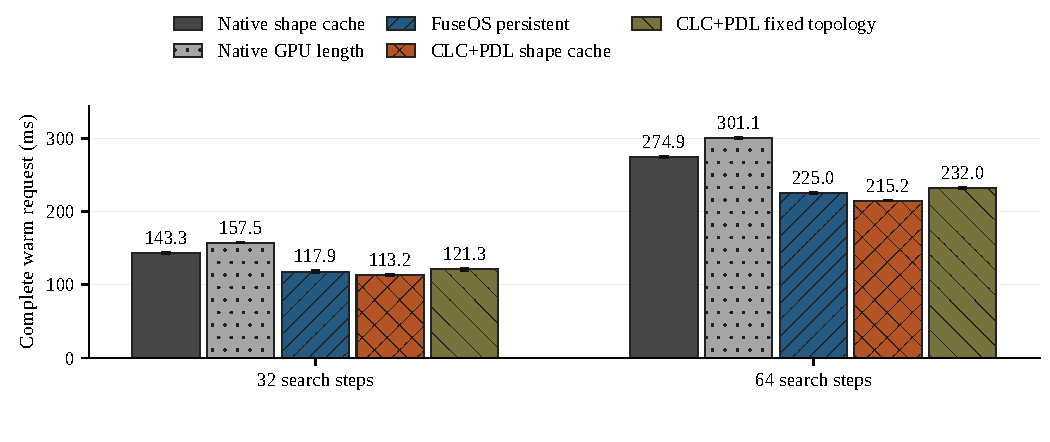
\includegraphics[width=\textwidth]{01_request.pdf}
\caption{\textbf{Complete Qwen3-0.6B requests after synchronization repair.}
Each request freshly prefills a 128-token ancestor and performs output-driven
search with at most four branches. Bars start at zero; whiskers span three
process medians (five requests per process). Shape-cache controls reuse all
encountered graphs; the fixed-topology control updates configuration without
recapture. All five methods produce the same final paths for each horizon.
The benefit over native execution includes the fused implementation as a
whole. Cached CLC+PDL remains a stronger executor than persistence here.}
\label{fig:request}
\end{figure*}

The FuseOS executor retains an application-level benefit after the attention repair.
For 32 search steps, the complete request takes \res{Persistent32}\,ms,
compared with \res{Native32}\,ms for native shape-cached execution
(\res{RequestGain32}$\times$). For 64 steps, the corresponding times are
\res{Persistent64}\,ms and \res{Native64}\,ms
(\res{RequestGain64}$\times$). Figure~\ref{fig:request} includes the native
GPU-length graph, which keeps graph count bounded by frontier width rather
than sequence depth. Thus the comparison is not against repeated Python
launches or compulsory graph reconstruction.

All 28 decoder layers and the vocabulary head execute in these intervals.
The searches expand 128 and 251 branch-tokens respectively; the latter
changes the live frontier between three and four branches. Both use model
outputs for parent/token selection, and the corrected custom paths reproduce
the final native candidate paths. The maximum request-gate NRMSE is
\res{MaxRequestNRMSE}, below the unchanged threshold.

\paragraph{What the positive result establishes.}
The complete dynamic executor is useful for this narrow-frontier workload.
The result does not isolate persistence from fused arithmetic. With the same
fused handlers, shape-cached CLC+PDL completes the two requests in
\res{CLC32}\,ms and \res{CLC64}\,ms, faster than the persistent executor.
The fixed-topology CLC+PDL control takes \res{Fixed32}\,ms and
\res{Fixed64}\,ms. This comparison distinguishes the cost of the execution
protocol from the benefit of the fused implementation. We retain the full
run ranges, including prefill variation, instead of presenting the small
fixed-topology differences as a universal persistent advantage.

\subsection{Dependence on workload geometry}
\label{sec:geometry}

\begin{figure*}[!tbp]
\centering
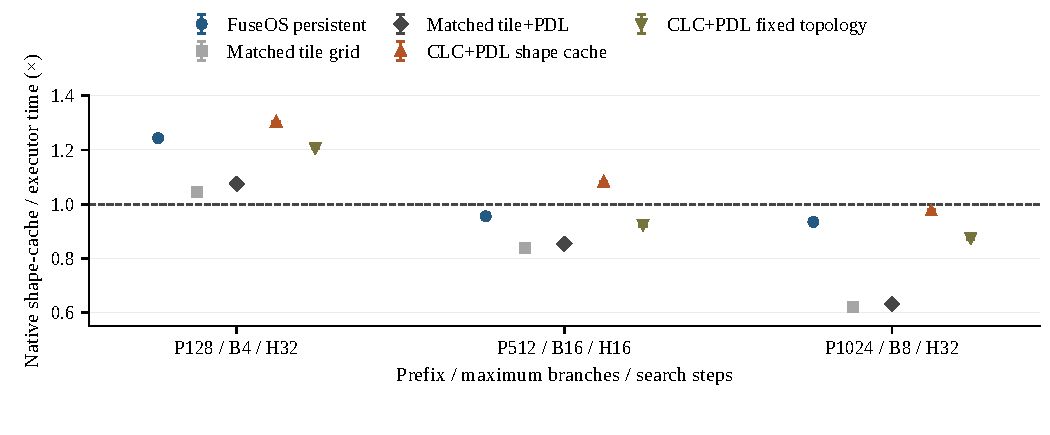
\includegraphics[width=\textwidth]{02_workload_boundary.pdf}
\caption{\textbf{Full-model equal-work search replay.} Native output-dependent
parent/token decisions are replayed for every backend while scoring still
executes inside timing. The interval starts from a ready prefilled ancestor;
it is not the complete-request interval in Figure~\ref{fig:request}. Higher
is faster; 1$\times$ is native shape-cached execution. Every point includes all
layers, KV updates, host policy, and synchronization. Points and whiskers are
the median and range of three round-indexed ratios.}
\label{fig:geometry}
\end{figure*}

We next hold the search trajectory constant to remove work differences from
the backend comparison. Three configurations vary ancestor length $P$,
maximum frontier width $B$, and horizon $H$: $(128,4,32)$, $(512,16,16)$, and
$(1024,8,32)$. Each uses a native-generated, output-dependent trace. All
qualified executors perform the same selected histories and execute the
selection policy during timing.

Figure~\ref{fig:geometry} shows that the narrow-frontier benefit does not
extend uniformly to wider or longer-prefix cases. Persistence improves on
the matched tile-grid and tile+PDL implementations, but native cached
execution becomes competitive or faster as workload geometry changes.
Shape-cached CLC+PDL provides another strong control. Since prefix, width,
horizon, and trajectory all change between cases, this figure defines an
observed applicability boundary rather than identifying a single causal
shape parameter. The maximum post-fix replay NRMSE is
\res{MaxReplayNRMSE}; timing includes no gate-failing configuration.



\subsection{Mechanism and larger-model controls}
Matched attention controls distinguish placement and task partitioning from
execution fusion. With identical 512-key jobs, replacing round-robin placement
with length-aware placement gives a geometric-mean
\res{placementGeo}$\times$ speedup and a maximum
\res{placementMax}$\times$. Changing an already sorted ordinary grid from
four partitions to finer 128-key jobs gives \res{partitionGeo}$\times$
geometrically, up to \res{partitionMax}$\times$. Both exploit information
known before dispatch. They must not be presented as evidence that a device
discovered new dynamic work more effectively.

The matched CLC phase-fusion control instead retains the same compiled entry,
task geometry, resources, and global exchange buffers, switching between
staged and last-producer reduction. Its geometric-mean increment is
\res{fusionGeo}$\times$. The change removes a launch but adds completion
and ordering work. Separate cluster-transport controls likewise do not
establish a large universal benefit from moving state across SMs. Their
implication for the OS design is to preserve good allocation and dataflow
plans before choosing a more elaborate execution mechanism.

The Qwen3.5-35B-A3B port provides another boundary. It covers routed MoE
work for microbatches of one to eight tokens and the DeltaNet decode path,
while other operations remain native. Its default fused path does not beat
native eager execution across the six evaluated workloads. Separating
selected stages reduces two request times from 721.11 to 682.92 ms and
from 554.12 to 547.39 ms. More fusion is therefore not an optimization
objective by itself. This separate mixed-Q4 comparison does not establish
BF16 accuracy or a port of every model operator to the new FX compiler.

\subsection{Slack sharing and its application boundary}
The resident-worker experiment runs independent 16$\times$16$\times$4096
BF16 GEMMs with FP32 accumulators, four warps per CTA. After a configurable
number $q$ of K tiles, each warp saves its accumulator and progress. The
foreground publishes an urgency flag on its own stream. Background workers
observe it at checkpoints but retain their allocations while paused.
Non-yielding long- and short-quantum controls isolate the effect of responding
to urgency from merely changing the amount of work in a quantum.

The streaming foreground contains eight independent BF16 GEMVs with
$M=2048$ and $K=8192$, reading 256 MiB of weights per step. Zero- and
100-$\mu$s device gaps provide distinct opportunities for background work.
This is not a transformer or a Kimi shard. The model foreground executes
all Qwen3-0.6B layers and the vocabulary head using native cached graphs,
with a 128-token prefix, up to four branches, and a 32-step native trace.
Unlike Figure 2, this sharing replay excludes search scoring; unlike
Figure 1, it excludes prefill. That distinction is preserved in the results.

Each configuration has an adjacent standalone reference, randomized order,
256 calibration steps, and 512 held-out steps in each of three fresh
processes. CUDA-event step latency includes the urgency markers and graph
execution but excludes the intentional gap. Background rate counts executed
K tiles over the host start-through-stop window, including startup, gaps,
submission, and the last slice drain. The artifact retains
\slackTimedSteps{} foreground timings including calibration and references.

% Generated by experiments/slack_scheduler/analyze.py; do not hand edit.
\begin{table*}[t]
\centering\small
\begin{tabular}{lrrrrr}
\toprule
Background policy & p50 cost (\%) & p99 cost (\%) [range] & TFLOP/s & Solo rate (\%) & Passes \\
\midrule
\multicolumn{6}{l}{\textit{Streaming GEMV proxy, 100-$\mu$s gaps}} \\
No yield, q4096, w64 & +22.06 & +23.68 [+23.64, +25.87] & 4.359 & 38.252 & 0/3 \\
No yield, q4, w64 & +18.70 & +20.91 [+20.77, +23.90] & 2.852 & 24.964 & 0/3 \\
Yield, q4, w64 & +0.58 & +0.62 [+0.58, +0.99] & 0.741 & 6.507 & 3/3 \\
Yield, q64, w64 & +2.34 & +2.50 [+2.32, +2.61] & 1.167 & 10.213 & 3/3 \\
Paced, q4, w32 & +1.17 & +1.16 [+1.15, +1.30] & 0.055 & 0.484 & 3/3 \\
\midrule
\multicolumn{6}{l}{\textit{Qwen3-0.6B native cached-graph decode replay}} \\
No yield, q4096, w64 & -1.80 & -1.57 [-1.67, -1.46] & 8.779 & 76.999 & 3/3 \\
No yield, q4, w64 & +4.44 & +3.92 [+1.36, +4.24] & 3.263 & 28.537 & 3/3 \\
Yield, q4, w64 & -3.40 & -4.42 [-4.47, -3.14] & 0.011 & 0.094 & 3/3 \\
Yield, q64, w64 & -3.25 & -3.04 [-4.44, -2.48] & 0.039 & 0.342 & 3/3 \\
Paced, q4, w32 & -1.58 & +0.37 [-1.51, +0.42] & 0.001 & 0.012 & 3/3 \\
\bottomrule
\end{tabular}
\caption{Co-running on RTX 5090. Values are medians of three paired process ratios; brackets are their ranges. Passes count held-out processes within the 6\% p99 budget. Solo rate is normalized to the fastest measured custom GEMM, not hardware peak. Here $q$ is K tiles per warp between checkpoints and $w$ is background CTAs, not reserved SMs.}
\label{tab:slack}
\end{table*}


With 100-$\mu$s gaps, the selected 64-worker, $q=64$ configuration provides
\slackProxyMediumRate{} TFLOP/s for \slackProxyMediumCost\% p99 cost.
Shorter $q=4$ checkpoints reduce cost to \slackProxyShortCost\% but provide
\slackProxyShortRate{} TFLOP/s. The long non-yielding control produces
\slackProxyLongRate{} TFLOP/s at \slackProxyLongCost\% cost and misses
the budget. Without an intentional gap, the selected configuration provides
\slackContinuousRate{} TFLOP/s at \slackContinuousCost\% cost; launch
and event boundaries still exist in that case.

The table's normalized rate uses the fastest measured configuration of the
same custom GEMM as its denominator. It is not a fraction of hardware peak
and cannot be compared numerically with another implementation's ``GPU
worth'' without matching its work and denominator. All nine frozen
calibration selections choose the 64-worker, $q=64$ policy, and all nine
pass held-out validation. Those observations do not establish generalization
to a new model, a new load trace, or a changed driver.

The full-model boundary is more important than the positive proxy point.
Whole-step suspension provides only \slackModelMediumRate{} TFLOP/s,
or \slackModelMediumFraction\% of the custom solo rate. The non-yielding
long-quantum control instead provides \slackModelLongRate{} TFLOP/s
while satisfying the observed p99 budget. It lacks a prompt-yield contract,
but it is a stronger performance control for that workload. The result
argues for phase-sensitive admission rather than protecting an entire model
step whenever a smaller interval would suffice. Negative measured latency
costs are retained under unlocked clocks and are not credited as a
scheduler-induced speedup.

\subsection{Checkpoint correctness and pause observations}
The handwritten worker checks all 256 outputs per warp and saved partial
accumulators against independent CPU arithmetic on binary-exact operands.
Resume tests include a quantum that leaves a partial GEMM. The streaming
outputs remain bitwise stable and selected rows pass an independent FP32
dot-product check. The final replay's model logits match the native reference
bitwise at every step. Bounded runs of the same worker entry pass memcheck,
racecheck, and synccheck with kernel filters. An initial live-worker sanitizer
attempt stalled and was terminated, so the bounded checks are not described
as certification of all concurrent execution.

A separate device probe measures urgency publication until all 64 workers
acknowledge suspension. Its p99 is \slackPauseShort{},
\slackPauseMedium{}, and \slackPauseLong{} $\mu$s for $q=4$, 64,
and 4096 respectively. The diagnostic polling kernel perturbs execution
and excludes CPU dispatch; its timings do not enter throughput aggregates.
Non-cooperative workers time out rather than acknowledging a yield.
The large change with quantum illustrates why block or slice lifetime is a
first-class admission cost.

The FX compiler has additional checks for broadcast/fan-out graphs, odd
matrix dimensions, FP32/FP16/BF16 arithmetic, linear/GELU compositions,
reductions and normalization, views, the \texttt{torch.compile} entry point,
and rejection/lifecycle behavior. Tests vary the program-count grant during
a partially completed reduction. Generated matrix, reduction, and pointwise
kernels pass separate bounded sanitizer checks. These establish correctness
for the supported cases; they do not imply coverage of arbitrary Python,
arbitrary CUDA kernels, training, or the complete Qwen graph.

\subsection{Existing hardware context switching}
The context-switch diagnostic deliberately uses non-cooperative work. A
background kernel launches one CTA on every SM, with more than half the
per-SM shared memory reserved so that only one such CTA can reside per SM.
Each CTA executes a 200-ms loop without an urgency poll. Its arithmetic
state and shared-memory sentinel are verified after completion. The foreground
probe reserves the same amount of shared memory, preventing it from being
explained by spare same-context residency.

\begin{table}[t]
\centering\small
\setlength{\tabcolsep}{3pt}
\begin{tabular}{lrrr}
\toprule
Probe placement & p50 (ms) & p99 (ms) & Full overlap \\
\midrule
Same context, high priority & 199.910 & 199.930 & 0/20 \\
Different CUDA process & 2.000 & 2.046 & 20/20 \\
\bottomrule
\end{tabular}
\caption{Warmed submission-to-completion latency for a 10-$\mu$s probe.
Full overlap means all 170 background CTA lifetimes enclose the complete
probe according to device timestamps. One process pair, 20 trials per mode.}
\label{tab:context}
\end{table}

The device advertises compute-preemption support. GPU timestamps and SM
identifiers confirm that, in every different-process trial, the probe runs
while all 170 background CTA lifetimes remain open. The corresponding
register computation and shared-memory state checks pass. In the same
context, higher stream priority does not interrupt the full-residency
background. These observations are consistent with driver-managed hardware
context preemption~\cite{CUDAComputePreemption}; they do not expose its
internal save format or measure the context-save operation in isolation.
The reported latency includes driver scheduling and submission overhead.

The process harness also runs one native Qwen foreground with one or three
compiler-generated GEMM background processes on this same device. Separate
contexts and a private MPS service are distinct configurations. Client PIDs
and MPS server attachment are recorded, and interrupted partial background
work is completed and checked after timing. The broader repeated process
sweep was paused during this paper's design-focused revision; partial rounds
are retained but are not used to assert an aggregate service-level speedup.
Single-device multiprocessing is not presented as multi-GPU reproduction.

\section{Hardware and Model Co-Design}
\label{sec:hardware}
The component results support the source paper's premise that software
scheduling and kernel design cannot by themselves manufacture every missing
device guarantee. We organize the hardware interface around three primary
requests and supporting observability and control services, following the
agenda of Nourai and Bastani~\cite{Nourai2026GPUOS}. These are requirements
of the proposed architecture, not capabilities claimed for the prototype.

\subsection{S1: bounded pause with state-preserving resume}
The desired primitive accepts a task or lease identifier, requests a pause,
and acknowledges within a specified time bound while preserving restart
state. Its contract must say whether it returns CTA resources, whether
memory transactions are drained, how barriers are preserved, and what
completion guarantees remain valid. A flag that stops useful issue without
returning allocation does not satisfy the same interface.

The source agenda's 5--20-$\mu$s target is substantially stronger than
observing that an independent CUDA process eventually runs. Our approximately
2-ms different-process probe latency is evidence that non-cooperative work
need not monopolize this device, but it is neither an application-selected
deadline nor a microsecond pause guarantee. Compiler-generated kernel
boundaries provide another usable control point, at the cost of submission,
checkpoint traffic, and lost locality. Both remain relevant even if future
hardware reduces one part of the revocation cost.

\subsection{S2: priority and rate control in shared memory paths}
SM separation alone cannot prevent L2 or DRAM interference. The desired
memory interface tags transactions by task class and supports policies for
urgent queueing, background rate limits, and observable enforcement. A
meaningful guarantee must distinguish bandwidth from latency and must define
the granularity at which priorities can change. Cache partitioning alone
does not provide a bound on memory-controller queueing delay.

The controller must also avoid starving traffic that is required for forward
progress. A background checkpoint or an outstanding write can be necessary
before resources become reclaimable. Treating all such traffic as indefinitely
deferrable can prevent the urgent lease from acquiring those resources.
The proposed tagging model includes dependency-critical completion traffic
and a bounded drain class in addition to foreground and background payloads.
The current CTA issue pacing does not implement this memory-controller policy.

\subsection{S3: enforceable per-kernel partitions}
The desired partition contract states which execution resources a kernel can
use and is honored consistently across ordinary launch, recorded graphs,
and changes of model phase. Static partitions can still be useful, but
rapidly alternating phases require either inexpensive partition changes or
a scheduler that selects appropriately provisioned queues. Merely accepting
a partition parameter in an API is not evidence that the physical execution
honors it.

A phase-dependent controller must account for its own transition cost.
Switching streams, queues, or contexts can introduce bubbles, synchronization,
and cache disruption. A promising single-layer result can consequently fail
when every layer pays the transition. The proposed planner evaluates complete
steps and includes partition transitions in the cost model. It does not add
the best isolated-phase throughput values and call the sum a feasible model
schedule.

\subsection{Supporting services and observability}
Priority inside an SM would complement, rather than replace, admission and
memory control. Urgent instructions sharing a resident allocation can still
be delayed by dependencies or transactions already issued by other work.
Fast device-wide signals and queues are useful when they have explicit
memory-ordering and progress guarantees. Accessible counters should separate
residency, arithmetic activity, traffic, and queueing instead of exposing one
ambiguous utilization number. Priority and pacing for copy engines, links,
and power complete the resource-vector interface.

\subsection{Models that produce predictable sharing opportunities}
Model architecture can make the scheduling problem easier without replacing
the OS contract. Balanced expert routing and similar expert sizes can reduce
phase variability. Linear-attention components can avoid some context-length
growth in the recurrent state update. Speculative or multi-token processing
can change the arithmetic reuse of a step. Each choice also changes numerical
semantics, latency, or memory use and must be evaluated with the actual model.
We do not infer a service speedup from regularity alone.

\section{Related Work and Scope}
\label{sec:related}
The resource-vector and slack-budget framing is directly inherited from
\emph{The GPU Needs an Operating System}; its large-model measurements and
hardware proposals motivate this specification~\cite{Nourai2026GPUOS}.
Our emphasis is the executable meaning of safe points, resource return,
publication, and admission, together with the boundaries visible in local
prototypes. Reframing those ideas as an API is not a claim of having invented
GPU sharing or having implemented the entire proposed stack.

FX provides the program-capture substrate and Triton the tiled code-generation
substrate~\cite{Reed2022FX,Tillet2019Triton}. The present compiler adds a
restricted checkpointed execution plan; it is not a replacement for either
general compiler framework. MPK combines a compiler and runtime for
mega-kernelizing tensor programs~\cite{Cheng2026MPK}. Meld couples dynamic
work placement, cross-SM cooperation, and just-in-time reduction
\cite{He2026Meld}. Our matched controls show why allocation, fusion, and
transport must be separated when attributing a speedup. Moving intermediate
data or claiming an unstarted CTA is not migration of a live program counter.

CUDA context scheduling, stream priorities, green contexts, and MPS are
lower-layer mechanisms with distinct contracts~\cite{CUDAStreams,CUDAGreen,NVIDIAMPS,CUDAComputePreemption}.
The architecture uses them where their documented guarantees match a lease.
It does not equate MPS clients with independent devices or a software memory
quota with hardware fault isolation. PagedAttention demonstrates the value
of treating KV allocation and sharing as first-class serving concerns
\cite{Kwon2023PagedAttention}; scheduling the compute that accesses those
pages requires additional lifetime and revocation rules.

\section{Limitations and Research Questions}
\label{sec:limits}
The complete object model remains an architectural specification. The current
artifact contains bounded fused inference, a restricted graph compiler,
cooperative workers, an IPC admission prototype, and diagnostics. It lacks
an integrated multi-tenant service, arbitrary-kernel transformation, a learned
interference predictor, a general memory-lease manager across protected
contexts, and the proposed hardware QoS controls. Correctness of supported
graphs and component numerical checks is not a proof of whole-system
isolation, fault recovery, or deadline satisfaction.

The measurements use one consumer Blackwell GPU with unlocked clocks.
They neither reproduce the source paper's RTX PRO 6000 model serving nor
establish transfer to AMD, TPU, SRAM-centric accelerators, or multi-node
deployments. Roofline reasoning can motivate those investigations, but
partition granularity, memory-system behavior, driver scheduling, and
communication must be remeasured on each target. In particular, the observed
context-switch diagnostic cannot specify a worst-case scheduling bound.

\section{Conclusion}
GPU sharing requires more than placing additional kernels beside a model.
It requires a contract for what work can stop, what state survives, what
resources are actually returned, and how much foreground slack admission
is allowed to spend. \system{} specifies that contract across processes,
compiler slices, resource leases, and hardware services. The component
evidence supports useful bounded execution and selected sharing opportunities,
while exposing costs that simpler utilization arguments miss. The architectural
goal is a general GPU operating system; the present contribution is a
specified path toward that goal with explicit implementation and evidence
boundaries.

\paragraph{Artifact and drafting disclosure.}
The repository includes raw timings, hashes, numerical checks, and build
instructions. Both figures retain qualified data; incomplete sweep rounds
are excluded from aggregate claims. AI-assisted tools supported code,
analysis, and prose. Results derive from retained measurement records.


\label{page:bodyend}
\clearpage
\bibliographystyle{plain}
\bibliography{references}
\end{document}
